% (C) Marc Lijour, 2017 
% Licensed under a Creative Commons License BY-SA
% https://creativecommons.org/licenses/by-sa/2.5/ca/
% Presentation for Ryerson University "Zone Learning Analytics School" (ZLAS) 
% authored by Marc Lijour, November 2017
% 
% ======================================================================================================
%                                     WHO AM I and OVERVIEW OF COLLIDERX
% ======================================================================================================
\section{ColliderX}
\frame{
        \tikz[remember picture,overlay] {
                \node(bkgd) at ([xshift=0cm,yshift=.3cm]current page.center)
                        {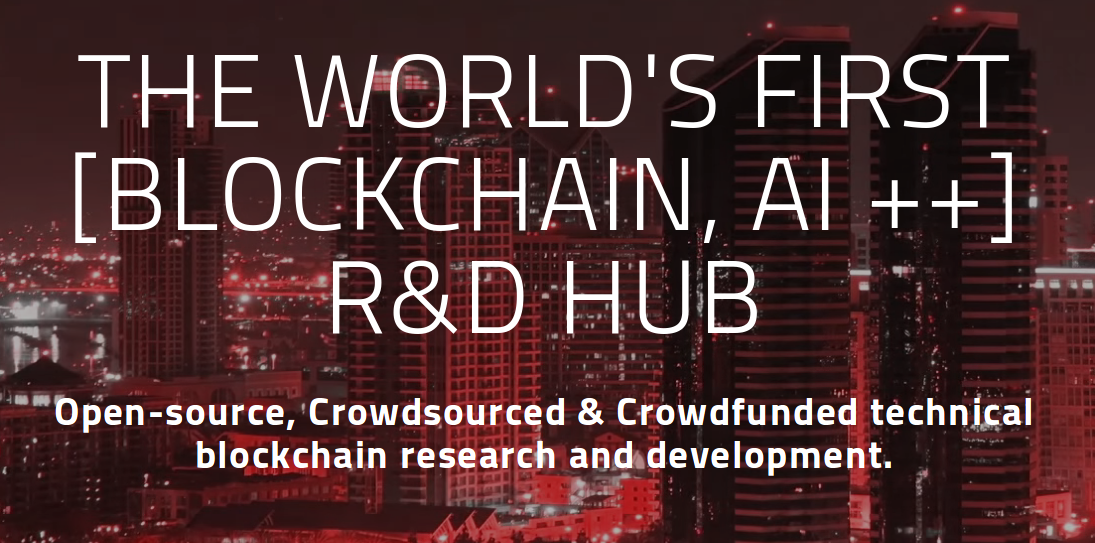
\includegraphics[width=\paperwidth]{../../pics/colliderx/colliderx-overview}};
        }
}

%\frame{
%	\frametitle{Présentateur}
%	\vspace{1.5em}
%	\begin{block}{Marc Lijour, Agent de changement dans le numérique}
%		Marc est le directeur exécutif du Centre national d'expertise sur le Blockchain, et co-fondateur de ColliderX.\\
%		\vspace{1em}
%		Après 7 ans d'expérience en tant qu'agent d'éducation au ministère de l'Éducation de l'Ontario, 
%		Marc a mené le secteur Éducation à Cisco Canada. Plus récemment, il représentait Savoir-faire Linux à Toronto.\\
%		\vspace{1em}
%		Marc siège au CA du CTIC, ainsi que d'autres organisations dont ColliderX, le Toronto French Business Network et TechConnex. 
%	\end{block}
%}

\frame{
	\frametitle{Mission: to accelerate the R\&D on Blokchain and related technologies}
	HOW\\
	\begin{itemize}
		\item infrastructure project proposal (\emph{need})
		\item backers (\$)
		\item researchers / developers (\emph{brains})
	\end{itemize}
}

\frame{
	\frametitle{Canadian Blockchain Supercluster}
	\begin{figure}
	
\includegraphics[width=11cm]{../../pics/colliderx/fabulousfive}
	\end{figure}
	\begin{itemize}
	        \item ColliderX, ICTC,  Blockchain Research Institute, and the two Canadian Blockchain associations 
		\item The five raised \$ 50 million in pledges under 3 weeks 
		\item Support for the shortlisted Supercluster proponents (ISED)
		\item Identified priorities: talent pipeline (education), regulation, start ups, R\&D in Canada, and more  
	\end{itemize}
}



